\documentclass[12pt]{article}            % Report class in 11 points
\parindent0pt  \parskip12pt             % make block paragraphs
\usepackage{graphicx}
\usepackage{listings}
\graphicspath{ {images/} }
\usepackage{graphicx} %  graphics header file
\begin{document}
\begin{titlepage}
    \centering
  \vfill
    
\includegraphics[width=8cm]{uni_logo.png} \\ 
	\vskip2cm
    {\bfseries\Large
	Data Structures and Algorithms \\ (CS09203)\\
	
	\vskip2cm
	Lab Report 
	 
	\vskip2cm
	}    

\begin{center}
\begin{tabular}{ l l  } 

Name: & Rehman ullah baig \\ 
Registration \#: &CSU-F16118 \\ 
Lab Report \#: & 11 \\ 
 Dated:& 2-07-2018\\ 
Submitted To:& Mr. Usman Ahmed\\ 

 %\hline
\end{tabular}
\end{center}
    \vfill
    The University of Lahore, Islamabad Campus\\
Department of Computer Science \& Information Technology
\end{titlepage}


    
    {\bfseries\Large
\centering
	Experiment \# 11 \\

The Kruskal's algorithm\\
	
	}    
 \vskip1cm
 \textbf {Objective}\\  To understand and implement The Kruskal's algorithm.
 
 \textbf {Software Tool} \\
1. Windows 7  \\
2. Dev C++\\
3. Miktex   \\

\section{Theory }              
Kruskal's algorithm is a minimum spanning tree algorithm that takes a graph as input and finds the subset of the edges of that graph which form a tree that includes every vertex has the minimum sum of weights among all the trees that can be formed from the graph.It falls under a class of algorithms called greedy algorithms which find the local optimum in the hopes of finding a global optimum.
We start from the edges with the lowest weight and keep adding edges until we we reach our goal.

The steps for implementing Kruskal's algorithm are as follows: \\

1. Sort all the edges from low weight to high.\\
2. Take the edge with the lowest weight and add it to the spanning tree. If adding the edge created a cycle, then reject this edge.\\
3. Keep adding edges until we reach all vertices.\\ \\

\section{Task}  
\subsection{Procedure: Task 1 }     

\begin{figure*}
\centering
  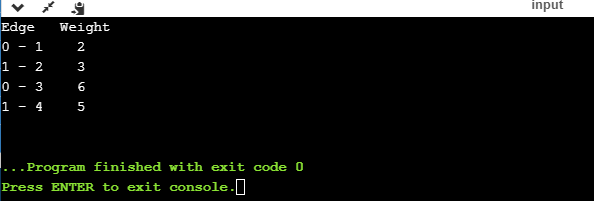
\includegraphics[width=12cm,height=6cm,keepaspectratio]{4.png}
\caption{Data entering into different locations}
\label{Figure:3}    
\end{figure*}
Kruskal's algorithm is a minimum-spanning-tree algorithm which finds an edge of the least possible weight that connects any two trees in the forest.[1] It is a greedy algorithm in graph theory as it finds a minimum spanning tree for a connected weighted graph adding increasing cost arcs at each step. This means it finds a subset of the edges that forms a tree that includes every vertex, where the total weight of all the edges in the tree is minimized. If the graph is not connected, then it finds a minimum spanning forest (a minimum spanning tree for each connected component).

\subsection{Procedure: Task 2 }     

\begin{lstlisting}[language=C++]


#include <iostream>
#include <stdio.h>
#include <limits.h>
#define V 5
using namespace std;
 

int minKey(int key[], bool mstSet[])
{
   int min = INT_MAX, min_index;
 
   for (int v = 0; v < V; v++)
     if (mstSet[v] == false && key[v] < min)
         min = key[v], min_index = v;
 
   return min_index;
}
 
int printMST(int parent[], int n, int graph[V][V])
{
   printf("Edge   Weight\n");
   for (int i = 1; i < V; i++)
      printf("%d - %d    %d \n", parent[i], i, graph[i][parent[i]]);
}
 

void primMST(int graph[V][V])
{
     int parent[V];
     int key[V];   
     bool mstSet[V];  
 
     for (int i = 0; i < V; i++)
        key[i] = INT_MAX, mstSet[i] = false;
 
  
     key[0] = 0;     
     parent[0] = -1; 
 
     for (int count = 0; count < V-1; count++)
     {
        
        int u = minKey(key, mstSet);
 
        mstSet[u] = true;
 
        for (int v = 0; v < V; v++)
 
          if (graph[u][v] && mstSet[v] == false && graph[u][v] <  key[v])
             parent[v]  = u, key[v] = graph[u][v];
     }

     printMST(parent, V, graph);
}
 
int main()
{

   int graph[V][V] = {{0, 2, 0, 6, 0},
                      {2, 0, 3, 8, 5},
                      {0, 3, 0, 0, 7},
                      {6, 8, 0, 0, 9},
                      {0, 5, 7, 9, 0},
                     };
 
   
    primMST(graph);
 
    return 0;
}
\end{lstlisting}

\section{Conclusion}  
we have covered the Intuitive idea behind the Kruskal algorithm and his computation complexity. Kruskal's algorithm is used in real world for map configuration.Kruskal’s algorithm is an “edge based algorithm”.  Prim’s algorithm with a heap is faster than Kruskal’s algorithm. Efficiency of Kruskal’s algorithm is based on the time needed for sorting the edge weights of a given graph
\end{document}                          % The required last line
